\usepackage{graphicx}%  A simple AAU report template.
%  2015-05-08 v. 1.2.0
%  Copyright 2010-2015 by Jesper Kjær Nielsen <jkn@es.aau.dk>

\documentclass[11pt,oneside,a4paper,openright]{report}
%%%%%%%%%%%%%%%%%%%%%%%%%%%%%%%%%%%%%%%%%%%%%%%%
% Language, Encoding and Fonts
% http://en.wikibooks.org/wiki/LaTeX/Internationalization
%%%%%%%%%%%%%%%%%%%%%%%%%%%%%%%%%%%%%%%%%%%%%%%%
% Select encoding of your inputs. Depends on
% your operating system and its default input
% encoding. Typically, you should use
%   Linux  : utf8 (most modern Linux distributions)
%            latin1 
%   Windows: ansinew
%            latin1 (works in most cases)
%   Mac    : applemac
% Notice that you can manually change the input
% encoding of your files by selecting "save as"
% an select the desired input encoding. 
\usepackage[utf8]{inputenc}
% Make latex understand and use the typographic
% rules of the language used in the document.
\usepackage[danish,english]{babel}
% Use the palatino font
\usepackage[sc]{mathpazo}
\linespread{1.05} % Palatino needs more leading (space between lines)
% Choose the font encoding
\usepackage[T1]{fontenc}
%%%%%%%%%%%%%%%%%%%%%%%%%%%%%%%%%%%%%%%%%%%%%%%%
% Graphics and Tables
% http://en.wikibooks.org/wiki/LaTeX/Importing_Graphics
% http://en.wikibooks.org/wiki/LaTeX/Tables
% http://en.wikibooks.org/wiki/LaTeX/Colors
%%%%%%%%%%%%%%%%%%%%%%%%%%%%%%%%%%%%%%%%%%%%%%%%
% Load a listings package
\usepackage{listings}
\lstloadlanguages{C,C++,csh,Java}
\lstset{aboveskip=20pt, belowskip=20pt}
\lstset{
language=csh,
basicstyle=\footnotesize\ttfamily,
numbers=left,
numberstyle=\tiny,
numbersep=5pt,
tabsize=2,
extendedchars=true,
breaklines=true,
frame=b,
stringstyle=\color{blue}\ttfamily,
showspaces=false,
showtabs=false,
xleftmargin=17pt,
framexleftmargin=17pt,
framexrightmargin=5pt,
framexbottommargin=4pt,
commentstyle=\color{green},
morecomment=[l]{//}, %use comment-line-style!
morecomment=[s]{/*}{*/}, %for multiline comments
showstringspaces=false,
morekeywords={ abstract, event, new, struct,
as, explicit, null, switch,
base, extern, object, this,
bool, false, operator, throw,
break, finally, out, true,
byte, fixed, override, try,
case, float, params, typeof,
catch, for, private, uint,
char, foreach, protected, ulong,
checked, goto, public, unchecked,
class, if, readonly, unsafe,
const, implicit, ref, ushort,
continue, in, return, using,
decimal, int, sbyte, virtual,
default, interface, sealed, volatile,
delegate, internal, short, void,
do, is, sizeof, while,
double, lock, stackalloc,
else, long, static,
enum, namespace, string},
keywordstyle=\color{cyan},
identifierstyle=\color{red},
backgroundcolor=\color{cloudwhite},
}
% load a colour package
\usepackage{xcolor}
\definecolor{aaublue}{RGB}{33,26,82}% Dark blue
\definecolor{red}{rgb}{0.6,0,0} 
\definecolor{blue}{rgb}{0,0,0.6}
\definecolor{green}{rgb}{0,0.8,0}
\definecolor{cyan}{rgb}{0.0,0.6,0.6}
\definecolor{cloudwhite}{rgb}{0.9412, 0.9608, 0.8471}
% The standard graphics inclusion package
\usepackage{graphicx}
% Set up how figure and table captions are displayed
\usepackage{caption}
\captionsetup{%
  font=footnotesize,% Set font size to footnotesize
  labelfont=bf % Bold label (e.g., Figure 3.2) font
}
% Make the standard latex tables look so much better
\usepackage{array,booktabs}
% Enable the use of frames around, e.g., theorems
% The framed package is used in the example environment
\usepackage{framed}

%%%%%%%%%%%%%%%%%%%%%%%%%%%%%%%%%%%%%%%%%%%%%%%%
% Mathematics
% http://en.wikibooks.org/wiki/LaTeX/Mathematics
%%%%%%%%%%%%%%%%%%%%%%%%%%%%%%%%%%%%%%%%%%%%%%%%
% Defines new environments such as equation,
% align and split 
\usepackage{amsmath}
% Adds new math symbols
\usepackage{amssymb}
% Use theorems in your document
% The ntheorem package is also used for the example environment
% When using thmmarks, amsmath must be an option as well. Otherwise \eqref doesn't work anymore.
\usepackage[framed,amsmath,thmmarks]{ntheorem}

%%%%%%%%%%%%%%%%%%%%%%%%%%%%%%%%%%%%%%%%%%%%%%%%
% Page Layout
% http://en.wikibooks.org/wiki/LaTeX/Page_Layout
%%%%%%%%%%%%%%%%%%%%%%%%%%%%%%%%%%%%%%%%%%%%%%%%
% Change margins, papersize, etc of the document
\usepackage[
  inner=28mm,% left margin on an odd page
  outer=28mm,% right margin on an odd page, i lowered this from 41 //Daniel
  ]{geometry}
% Modify how \chapter, \section, etc. look
% The titlesec package is very configureable
\usepackage{titlesec}
% Section
\titleformat{\section}
  {\normalfont\LARGE\bfseries}{\thesection}{1em}{}[{\hrule}]
% Subsection
\titleformat{\subsection}
  {\normalfont\Large\bfseries}{\thesubsection}{1em}{}[{}]
% Subsubsection 
\titleformat{\subsubsection}
  {\normalfont\large\bfseries}{\thesection}{1em}{}[{\smallskip}]

%\titleformat{\chapter}[display]{\normalfont\huge\bfseries}{\chaptertitlename\ \thechapter}{20pt}{\Huge}
%\titleformat*{\section}{\normalfont\Large\bfseries}
%\titleformat*{\subsection}{\normalfont\large\bfseries}
%\titleformat*{\subsubsection}{\normalfont\normalsize\bfseries}
%\titleformat*{\paragraph}{\normalfont\normalsize\bfseries}
%\titleformat*{\subparagraph}{\normalfont\normalsize\bfseries}

% Clear empty pages between chapters
\let\origdoublepage\cleardoublepage
\newcommand{\clearemptydoublepage}{%
  \clearpage
  {\pagestyle{empty}\origdoublepage}%
}
\let\cleardoublepage\clearemptydoublepage

% Change the headers and footers
\usepackage{fancyhdr}
\pagestyle{fancy}
\fancyhf{}% Delete everything
\setlength{\headheight}{14pt}
\renewcommand{\headrulewidth}{0pt} % Remove the horizontal line in the header
\fancyhead[RE]{\small\nouppercase\leftmark}% Even page - chapter title
\fancyhead[LO]{\small\nouppercase\rightmark}% Uneven page - section title
\fancyhead[LE,RO]{\thepage}% Page number on all pages
% Do not stretch the content of a page. Instead,
% insert white space at the bottom of the page
\raggedbottom
% Enable arithmetics with length. Useful when
% typesetting the layout.
\usepackage{calc}

%%%%%%%%%%%%%%%%%%%%%%%%%%%%%%%%%%%%%%%%%%%%%%%%
% Bibliography
% http://en.wikibooks.org/wiki/LaTeX/Bibliography_Management
%%%%%%%%%%%%%%%%%%%%%%%%%%%%%%%%%%%%%%%%%%%%%%%%
\usepackage{csquotes} % Somehow this has to be here when using babel package //Daniel
\usepackage[style=ieee]{biblatex}
\addbibresource{bib/mybib.bib}

%%%%%%%%%%%%%%%%%%%%%%%%%%%%%%%%%%%%%%%%%%%%%%%%
% Appendices
\usepackage[toc,page]{appendix}
\renewcommand{\appendixtocname}{Bilag}
\renewcommand{\appendixpagename}{Bilag}
%%%%%%%%%%%%%%%%%%%%%%%%%%%%%%%%%%%%%%%%%%%%%%%%

%%%%%%%%%%%%%%%%%%%%%%%%%%%%%%%%%%%%%%%%%%%%%%%%
% Misc
%%%%%%%%%%%%%%%%%%%%%%%%%%%%%%%%%%%%%%%%%%%%%%%%
% Add bibliography and index to the table of
% contents
\usepackage[nottoc]{tocbibind}
% Add the command \pageref{LastPage} which refers to the
% page number of the last page
\usepackage{lastpage}
% Add todo notes in the margin of the document
\usepackage[
% Disable, % turn off todonotes
  colorinlistoftodos, % Enable a coloured square in the list of todos
  textwidth=\marginparwidth, % Set the width of the todonotes
  textsize=scriptsize, % Size of the text in the todonotes
  ]{todonotes}

%%%%%%%%%%%%%%%%%%%%%%%%%%%%%%%%%%%%%%%%%%%%%%%%
% Hyperlinks
% http://en.wikibooks.org/wiki/LaTeX/Hyperlinks
%%%%%%%%%%%%%%%%%%%%%%%%%%%%%%%%%%%%%%%%%%%%%%%%
% Enable hyperlinks and insert info into the pdf
% file. Hypperref should be loaded as one of the 
% last packages
\usepackage{hyperref}
\hypersetup{%
	%pdfpagelabels=true,%
	plainpages=false,%
	pdfauthor={Author(s)},%
	pdftitle={Title},%
	pdfsubject={Subject},%
	bookmarksnumbered=true,%
	colorlinks=false,%
	citecolor=black,%
	filecolor=black,%
	linkcolor=black,% You should probably change this to black before printing
	urlcolor=black,%
	pdfstartview=FitH%
}

% Daniels legeplads
\setlength{\parindent}{0pt}% Package inclusion and set up of the document
% See, e.g., http://en.wikibooks.org/wiki/LaTeX/Formatting#Hyphenation
% for more information on word hyphenation
\hyphenation{ex-am-ple hy-phen-a-tion short}
\hyphenation{long la-tex}% 
\newcommand{\aautitlepage}[3]{%
  {
    % Set up various length
    \ifx\titlepageleftcolumnwidth\undefined
      \newlength{\titlepageleftcolumnwidth}
      \newlength{\titlepagerightcolumnwidth}
    \fi
    \setlength{\titlepageleftcolumnwidth}{0.5\textwidth-\tabcolsep}
    \setlength{\titlepagerightcolumnwidth}{\textwidth-2\tabcolsep-\titlepageleftcolumnwidth}
    % Create title page
    \thispagestyle{empty}
    \noindent%
    \begin{tabular}{@{}ll@{}}
      \parbox{\titlepageleftcolumnwidth}{
        \iflanguage{danish}{%
          %\includegraphics[width=\titlepageleftcolumnwidth]{figures/aau_logo_da}
        }{%
          %\includegraphics[width=\titlepageleftcolumnwidth]{figures/aau_logo_en}
        }
      } &
      \parbox{\titlepagerightcolumnwidth}{\raggedleft\sf\small
        #2
      }\bigskip\\
       #1 &
      \parbox[t]{\titlepagerightcolumnwidth}{%
      \textbf{Abstract:}\bigskip\par
        \fbox{\parbox{\titlepagerightcolumnwidth-2\fboxsep-2\fboxrule}{%
          #3
        }}
      }\\
    \end{tabular}
    \vfill
    \iflanguage{danish}{%
      \noindent{\footnotesize\emph{Rapportens indhold er frit tilgængeligt, men offentliggørelse (med kildeangivelse) må kun ske efter aftale med forfatterne.}}
    }{%
      \noindent{\footnotesize\emph{The content of this report is freely available, but publication (with reference) may only be pursued due to agreement with the author.}}
    }
    \clearpage
  }
}

% Create danish project info
\newcommand{\danishprojectinfo}[8]{%
  \parbox[t]{\titlepageleftcolumnwidth}{
    \textbf{Titel:}\\ #1\bigskip\par
    \textbf{Tema:}\\ #2\bigskip\par
    \textbf{Projektperiode:}\\ #3\bigskip\par
    \textbf{Projektgruppe:}\\ #4\bigskip\par
    \textbf{Deltager(e):}\\ #5\bigskip\par
    \textbf{Vejleder(e):}\\ #6\bigskip\par
    \textbf{Oplagstal:} #7\bigskip\par
    \textbf{Sidetal:} \pageref{LastPage}\bigskip\par
    \textbf{Afleveringsdato:}\\ #8
  }
}% My macros

\begin{document}

% Translate word that are english by default, to danish
\addto\captionsenglish{
   \renewcommand\chaptername{Kapitel} 
   \renewcommand{\figurename}{Figur}
   \renewcommand{\bibname}{Litteraturliste}
   \renewcommand{\contentsname}{Indholdsfortegnelse}
   \renewcommand{\tablename}{Tabel}
   \renewcommand{\appendixname}{Bilag}
} 

% Frontmatter
\pagestyle{empty}% Disable headers and footers
\pagenumbering{roman}% Use roman page numbering in the frontmatter
\pdfbookmark[0]{Front page}{label:frontpage}%
\begin{titlepage}
  \addtolength{\hoffset}{0.5\evensidemargin-0.5\oddsidemargin}% Set equal margins on the frontpage - remove this line if you want default margins
  \noindent%
  \begin{tabular}{@{}p{\textwidth}@{}}
    \toprule[2pt]
    \midrule
    \vspace{0.2cm}
    \begin{center}
    \Huge{\textbf{
      Biograf Nordic % Insert your title here
    }}
    \end{center}
    \begin{center}
      \Large{
        - Rapport i programmering og teknologi - % Insert your subtitle here
      }
    \end{center}
    \vspace{0.2cm}\\
    \midrule
    \toprule[2pt]
  \end{tabular}
  \vspace{4 cm}
  \begin{center}
    {\large
      3. semester % Insert document type (e.g., Project Report)
    }\\
    \vspace{0.2cm}
    {\Large
      Gruppe 1, Dmab0919 % Insert your group name or real names here
    }
  \end{center}
  \vfill
  \begin{center}
  Professionshøjskolen UCN\\
  Datamatiker
  \end{center}
\end{titlepage}
\clearpage
\thispagestyle{empty}
{\small
\strut\vfill % Push the content to the bottom of the page
\noindent Copyright \copyright{} Professionshøjskolen UCN 2020\par
\vspace{0.2cm}
\noindent % Write something if relevant
}
\clearpage
\cleardoublepage
{\selectlanguage{danish}
\pdfbookmark[0]{Danish title page}{label:titlepage_da}
\aautitlepage{%
  \danishprojectinfo{
    Biograf Nordic % Title
  }{%
    Agil udvikling % Theme
  }{%
    Efterårssemestret 2020 % Project period
  }{%
    Gruppe 1 % Project group
  }{%
    % List of group members
    Daniel Thomsen\\ 
    Jesper Mellergaard\\
    Kasper Møller Nielsen\\
    Kristoffer Aagard Mikkelsen
  }{%
    % List of supervisors
    Henrik Kristian Ulrik Øllgaard
  }{%
    1 % Number of printed copies
  }{%
    21. december 2020 % Date of completion
  }%
}{% Department and address
  \textbf{Datamatiker}\\
  Professionshøjskolen UCN\\
  Sofiendalsvej 60\\
  \href{http://www.ucn.dk}{http://www.ucn.dk}
}{% The Abstract
  Her er resuméet
}}
\chapter*{Forord\markboth{Forord}{Forord}}\label{ch:forord}
Denne rapport er udarbejdet af en gruppe studerende på 3. semester på datamatikeruddannelsen på University College Nordjylland pr. 2020 \\

Til dette projektforløb har gruppen skulle skrive to seperate rapporter. Denne rapport har til formål at dokumentere alt relevant til systemudvikling.
Herunder gælder at redegøre for forskellige procesmodeller og udviklingsmetoder, hvorefter at dokumentere hvordan projektgruppen aktivt har arbejdet med disse.
Envidere vil gruppen overvejelser i forhold til arkitektur og risikohåndtering blive dokumenteret. \\

Som elektronisk bilag til begge rapporter, er det biograf booking system blevet udviklet. Til udvikling af systemet er følgende værktøjer blevet brugt:

\begin{itemize}
    \item C\# til back-end programmering, og Vue til front-end.
    \item MS-SQL Database.
    \item Github til versionsstyring.
    \item Scrum og XP som udviklingsmetode, og YouTrack som scrum-værktøj.
\end{itemize}

Gruppen har i projektforløbet fået tildelt systemudviklingsunderviser Henrik Kristian Ulrik Øllgaard, 
til at vejlde i forbindelse med systemudviklingsrapporten.

\vspace{\baselineskip}\hfill Professionshøjskolen UCN, \today

\vfill\noindent
\begin{minipage}[b]{0.45\textwidth}
 \centering
 \rule{\textwidth}{0.5pt}\\
  Daniel Thomsen\\
 {\footnotesize <1080612@ucn.dk>}
\end{minipage}
\hfill
\begin{minipage}[b]{0.45\textwidth}
 \centering
 \rule{\textwidth}{0.5pt}\\
  Jesper Mellergaard\\
 {\footnotesize <1080645@ucn.dk>}
\end{minipage}
\vspace{3\baselineskip}
\newline
\begin{minipage}[b]{0.45\textwidth}
 \centering
 \rule{\textwidth}{0.5pt}
  Kasper Møller Nielsen\\
 {\footnotesize <1080649@ucn.dk>}
\end{minipage}
\hfill
\begin{minipage}[b]{0.45\textwidth}
 \centering
 \rule{\textwidth}{0.5pt}\\
 Kristoffer Aagard Mikkelsen\\
 {\footnotesize <1080659@ucn.dk>}
\end{minipage}
\newpage
\section*{Læsevejledning}
\cleardoublepage
\pdfbookmark[0]{Contents}{label:contents}
\pagestyle{fancy}% Enable headers and footers again
\tableofcontents
\cleardoublepage

% Mainmatter
% Intro
\pagenumbering{arabic}% Use arabic page numbering in the mainmatter
Dette kapitel har til formål at redegøre for systemets opbygning, samt klargøre hvilke valg 
der er blevet taget i forhold til systemets arkitektur. Hertil bliver der også fremvist Domanemodel, 
design klassediagram af api'et og relationmodeldiagram af databasen for at give indblik i de konkrete klasser.

% Body
\chapter{Procesmodeller}\label{ch:procesmodeller}
Dette kapitel har til formål at redegøre for systemets opbygning, samt klargøre hvilke valg 
der er blevet taget i forhold til systemets arkitektur. Hertil bliver der også fremvist Domanemodel, 
design klassediagram af api'et og relationmodeldiagram af databasen for at give indblik i de konkrete klasser.
\section{Vandfaldsmetoden}\label{sec:vandfald}
Vandfalds-modellen er en sekventiel procesmodel som består af 5-7 forskellige faser. 
Navnet vandfald er blevet brugt, da det ikke er muligt at vende tilbage til foregående faser, 
når først en fase er færdiggjort. Resultatet fra hver fase er et krav for at kunne starte på den næste. 
Hvis kunden kommer med store ændringer til kravene, bliver hele processen nødt til at starte forfra.  
Vandfalds-modellen kan ses på Figur \ref{fig:waterfallmodel} \\

\begin{figure}[h]
    \centering
    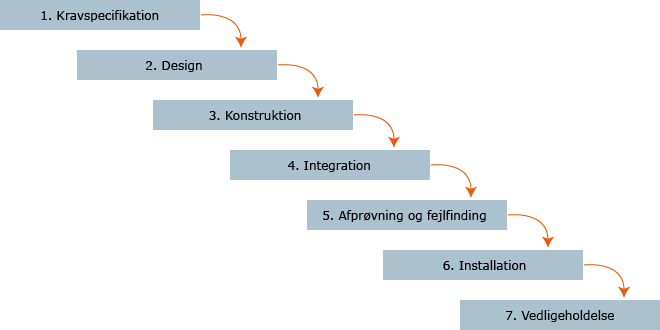
\includegraphics[width=0.7\textwidth]{figures/waterfall.png}
    \caption{Vandfaldsmodellen \cite{WaterfallModel}}
    \label{fig:waterfallmodel}
\end{figure}

Denne metode kan virke godt I forbindelse med mindre projekter, hvor det afsluttende produkt er 
helt defineret og det ikke forventes at ændringer kan forekomme. Hvis projektet er for stort og kompliceret,
kan det ofte medføre, at der på sigt vil være ændringer i enten arkitekturen eller selve funktionaliteten.
Dette tager vandfaldsmodellen ikke højde for.

\section{Agile metoder}\label{sec:agilemetoder}
Agil er en betegnelse for en række iterative softwareudviklingsmetoder, hvor der løbende leveres små dele af 
produktet til kunden. Agile udviklingsmetoder er oftest kendetegnet ved Det Agile Manifest \cite{AgileManifesto}.
Manifestet beskriver blandt andet hvordan samtaler og møder med kunden, samt god, fungerende software er i fokus, 
fremfor en lang liste af processer og værktøjer og fuldstændig dokumentation. \\

Ved udvikling af større softwaresystemer, hvor kunden er en nær kontakt igennem udviklingsperioden, kan udviklerteamet
drage stor fordel af at udvikle agilt. Dette skyldes at agile metoder bygger på \textit{continual improvement},
hvilket vil sige at produktet bliver udviklet inkrementelt, sådan at man altid har noget at vise kunden. Desuden er en fordel ved agile
metoder at de er omstillingsparate. Dette skyldes at man kun planlægger sit arbejde få uger frem.

\chapter{Udviklingsværktøjer}\label{ch:udviklingsvaerktoejer}
Dette kapitel har til formål at redegøre for systemets opbygning, samt klargøre hvilke valg 
der er blevet taget i forhold til systemets arkitektur. Hertil bliver der også fremvist Domanemodel, 
design klassediagram af api'et og relationmodeldiagram af databasen for at give indblik i de konkrete klasser.
\section{Scrum}\label{sec:scrum}

\section{XP}\label{sec:xp}

\section{Kanban}\label{sec:kanban}

\section{Metodevalg}\label{sec:valgafvaektoej}

\chapter{Udviklingen}\label{ch:udviklingen}
Dette kapitel har til formål at redegøre for systemets opbygning, samt klargøre hvilke valg 
der er blevet taget i forhold til systemets arkitektur. Hertil bliver der også fremvist Domanemodel, 
design klassediagram af api'et og relationmodeldiagram af databasen for at give indblik i de konkrete klasser.
\section{Brug af scrum}\label{sec:brugafscrum}

\subsection{Sprint 0}

% Outro
\chapter{Konklusion}\label{ch:konklusion}
\chapter{Refleksion}\label{ch:refleksion}

% Endmatter?
\printbibliography[heading=bibintoc]
\label{bib:mybiblio}
\begin{appendices}
\chapter{Første bilag}\label{app:foerstebilag}
Et bilag
\end{appendices}
\end{document}